\subsection{Коррекция перспективы}

Коррекция перспективы необходима для устранения шума на изображении и получения лучшего результата. 
В данной работе коррекция перспективы осуществляется при помощи библиотеки для обработки изображений $OpenCV$. Использование данной библиотеки обладает следующими преимуществами:
\begin{itemize}
    \item Простота внедрения: $OpenCV$ предоставляет готовые функции для коррекции перспективы, например, $cv2.warpPerspective$ \cite{opencv_perspective_transform}.
    \item Отсутствие необходимости в больших данных для обучения.
    \item Детерминированность: результат всегда является детерминированным, так как основан на точных математических алгоритмах.
    \item Производительность: библиотека написана на производительном языке $C++\;$ с использованием различных оптимизаций.
    \item Небольшие вычислительные затраты: по сравнению с нейросетевыми моделями, использование $OpenCV$ требует значительно меньших ресурсов.
    \item Поддержка различных платформ: библиотека является кросс-платформенной и поддерживает основные платформы, такие как $Windows$, $Linux$, $macOS$, $Android$, $iOS$.
    \item Поддержка и документация: $OpenCV$ обладает широким сообществом, а также обширной документацией с примерами использования тех или иных алгоритмов.
\end{itemize}

Сам алгоритм коррекции перспективы состоит из нескольких этапов, представленных на рисунке~\ref{perspective_correction_algo}. 

Необходимо подчеркнуть, что процесс коррекции перспективы базируется исключительно на алгоритмах анализа изображений без привлечения сложных алгоритмов нейросетевого обучения.
Поэтому в целях экономии ресурсов сервера, а в следствии улучшения производительности, было принято решение выполнять данный этап на ЭВМ клиента.
\begin{figure}
    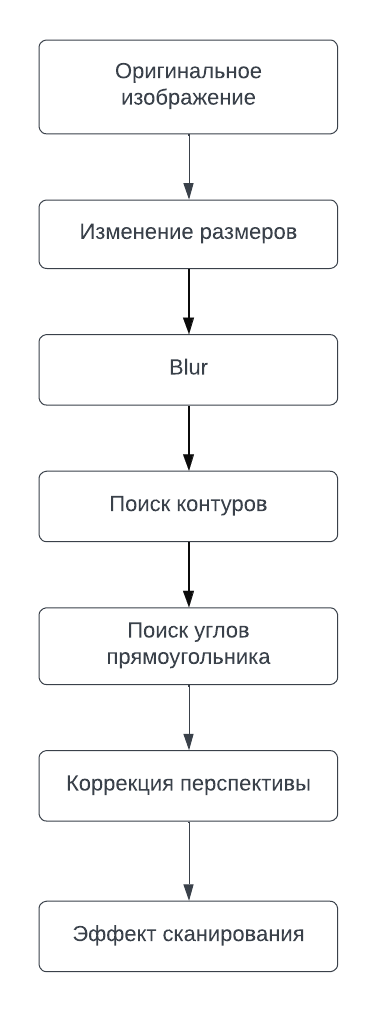
\includegraphics[scale=0.75]{img/perspective_correction.png}
    \caption{Этапы коррекции перспективы изображения}
    \label{perspective_correction_algo}
\end{figure}

На начальном этапе мы имеем изображение, показанное на рисунке~\ref{input}.

\begin{figure}
    \begin{turn}{270}
        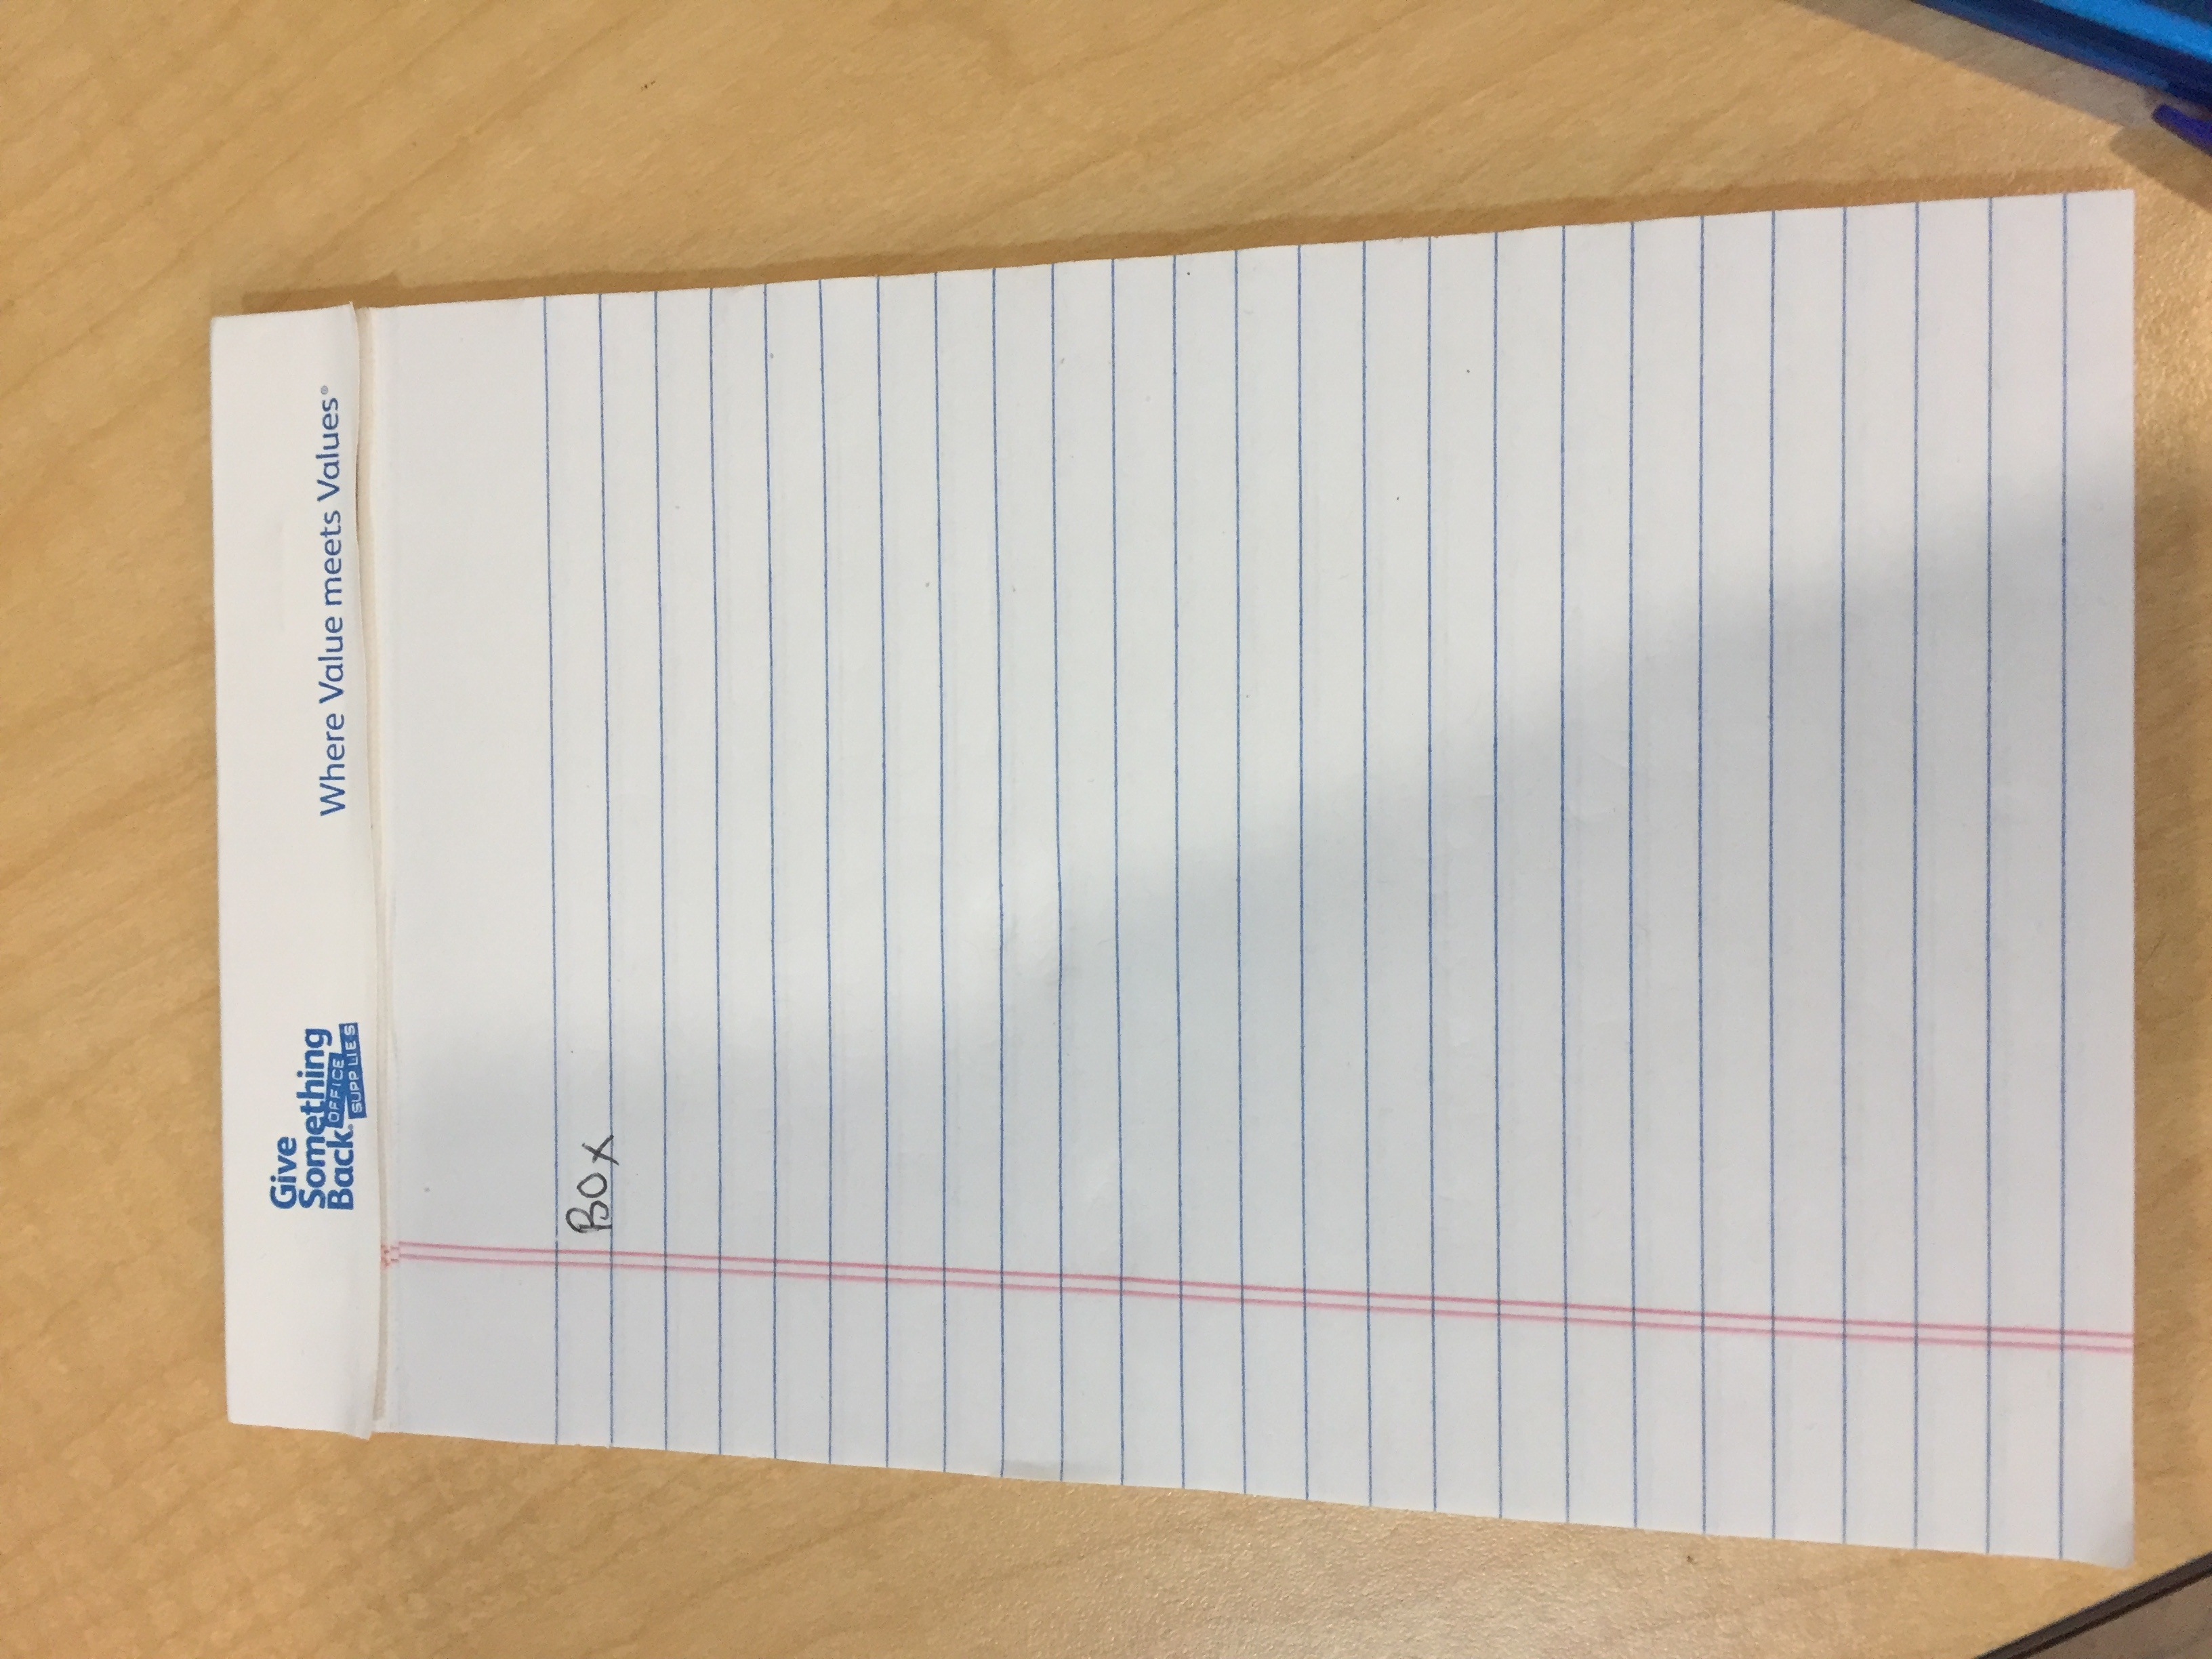
\includegraphics[scale=0.05]{img/perspective/input.JPG}
    \end{turn}
    \caption{Начальное изображение}
    \label{input}
\end{figure}

Для начала необходимо удалить текст с изображения. Для этого преобразуем изображение в серый цвет и применим к нему размытие Гаусса \cite{gauss_blur}. На выходе данного этапа имеем изображение, представленное на рисунке~\ref{gauss_blur}.

\begin{figure}
    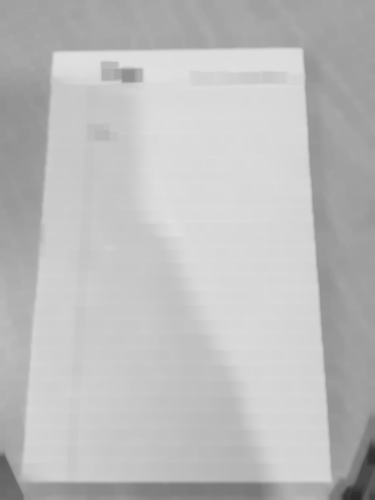
\includegraphics[scale=0.25]{img/perspective/blured.png}
    \caption{Изображение после размытия Гаусса}
    \label{gauss_blur}
\end{figure}

Для поиска контуров необходимо выделить ребра. Для этого используется алгоритм Канни \cite{canny}. На выходе имеем изображение, представленное на рисунке~\ref{canny}.
\begin{figure}
    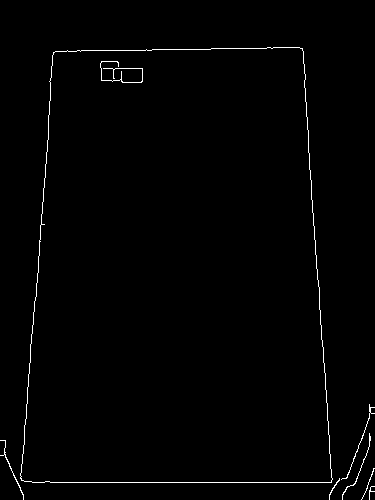
\includegraphics[scale=0.25]{img/perspective/canny.png}
    \caption{Ребра, найденные на изображении}
    \label{canny}
\end{figure}

После нахождения ребер поиск контуров осуществляется двумя способами:
\begin{enumerate}
    \item с помощью алгоритма $Line\;Segment\;Detector$ \cite{lsd};
    \item с помощью встроенного в $OpenCV$ алгоритма поиска контуров \cite{opencv_contours}.
\end{enumerate}

Опишем подробнее поиск контуров на основе найденных линий: после прохода алгоритма имеем изображение, представленное на рисунке~\ref{lsd_img}.
\begin{figure}
    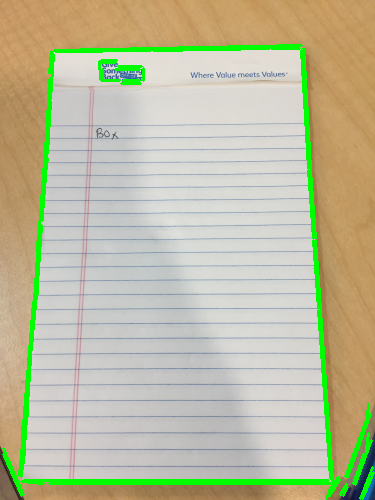
\includegraphics[scale=0.25]{img/perspective/lsd.png}
    \caption{Найденные на изображении линии с помощью алгоритма $LSD$}
    \label{lsd_img}
\end{figure}

Контур определяется как пересечение горизонтальных и вертикальных линий. На выходе имеем найденные углы контура, показанные на рисунке ~\ref{lsd_corners}.
\begin{figure}
    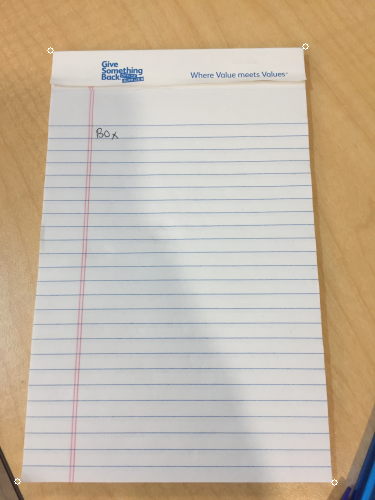
\includegraphics[scale=0.25]{img/perspective/corners.png}
    \caption{Найденные на изображении контуры на основе линий}
    \label{lsd_corners}
\end{figure}

С помощью библиотеки $OpenCV$ контуры находятся следующим образом:

\begin{enumerate}
    \item находятся 5 наибольших по площади контуров;
    \item найденные контуры проверяются на количество углов, минимальную площадь контура.
\end{enumerate}

Среди всех подходящих контуров выбирается наибольший по площади, как показано на рисунке ~\ref{contours}.
\begin{figure}
    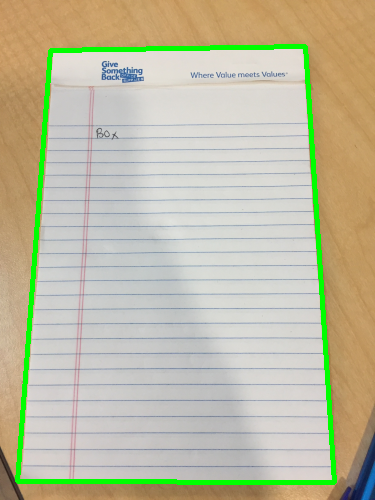
\includegraphics[scale=0.25]{img/perspective/contours.png}
    \caption{Найденные алгоритмом контуры}
    \label{contours}
\end{figure}


На основе найденного контура, представляющего лист бумаги, осуществляем коррекцию перспективы. Для этого находим матрицу коррекции \cite{opencv_perspective_transform} и примянем ее к изображению \cite{opencv_warp_perspective}.
Получаем результирующее изображение, показанное на рисунке ~\ref{perspective_correction}.
\begin{figure}
    \includegraphics[scale=0.05]{img/perspective/perspective.png}
    \caption{Изображение с коррекцией перспективы}
    \label{perspective_correction}
\end{figure}

Далее необходимо добавить эффект сканирования. Эффект достигается путем применения к композиции небольшого размытия и серого изображения алгоритма сегментации $Adaptive\;Threshold$ \cite{opencv_threshold}. 
В конечном итоге имеем результирующее изображение показанное на рисунке ~\ref{preprocess_out}.

\begin{figure}
    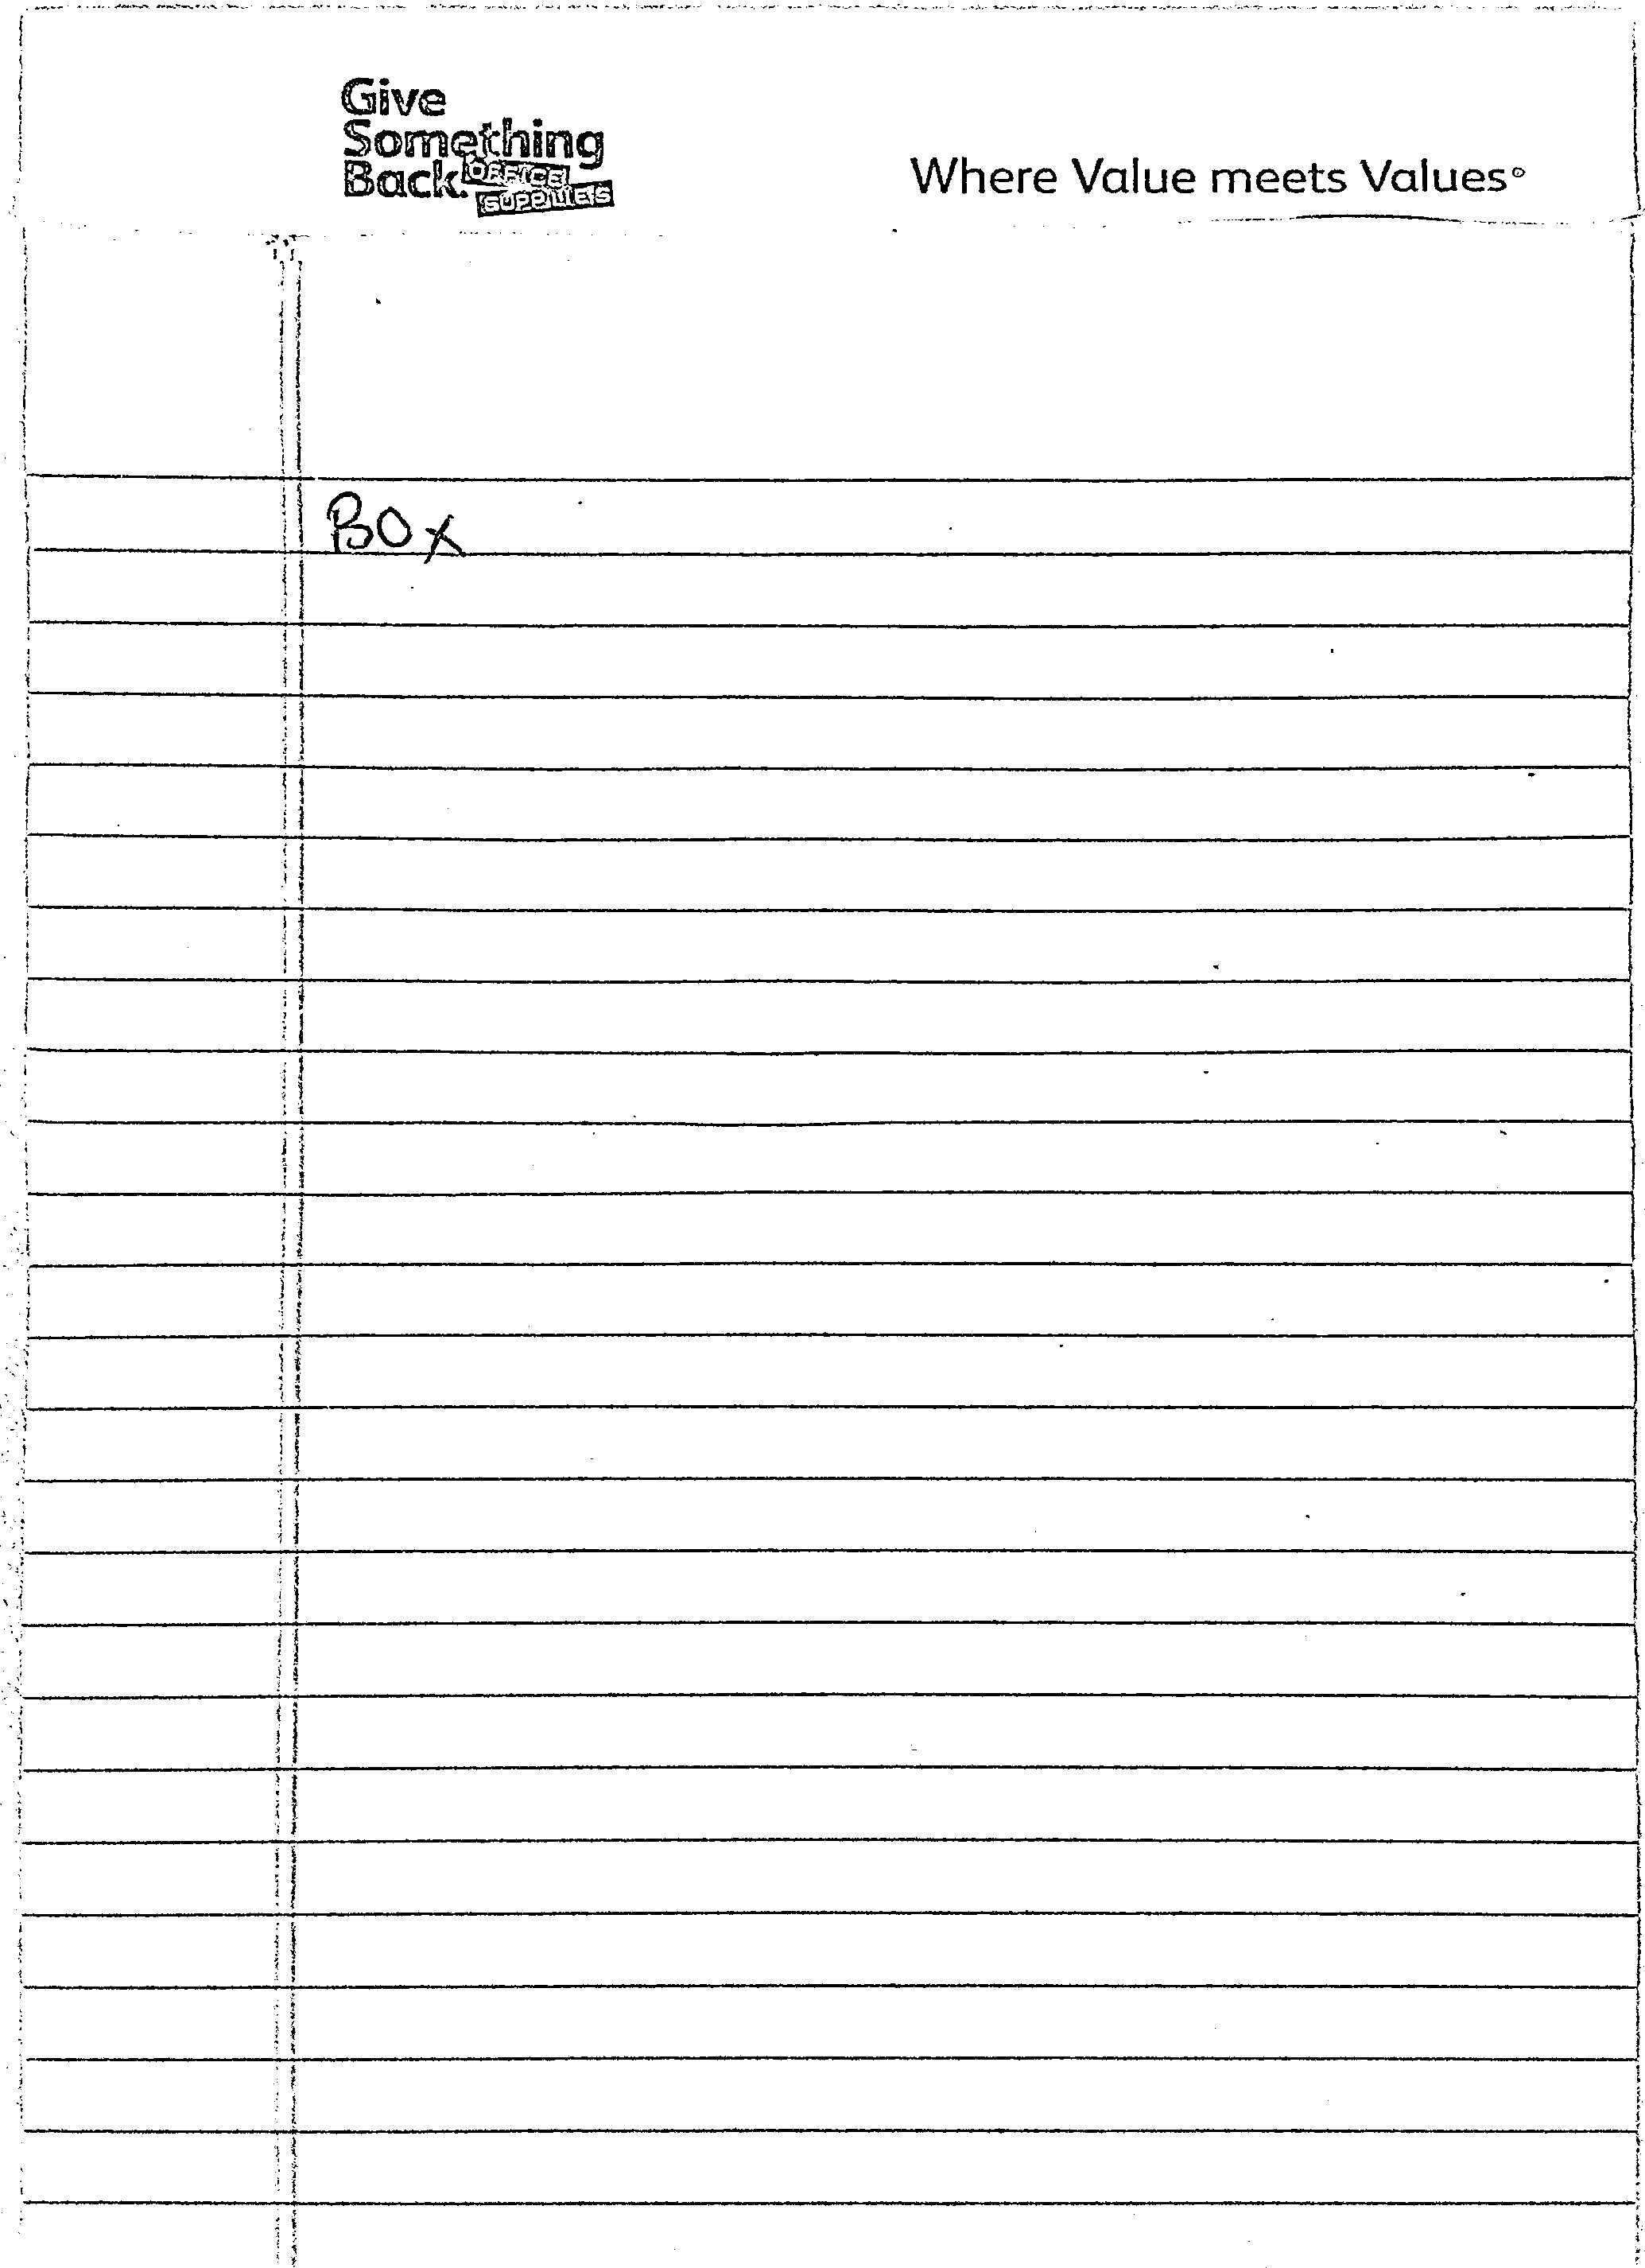
\includegraphics[scale=0.05]{img/perspective/output.JPG}
    \caption{Результирующее изображение}
    \label{preprocess_out}
\end{figure}

\subsubsection{Неправильное распознавание}
Стоит отметить, что данный алгоритм не является универсальным. Например, если на изображении находится посторонний шум (например, палец на бумаге, экран монитора, большое здание в виде прямоугольника), 
то вероятность получения неверного результата кратно возрастает. Именно с целью защиты от таких случаев в конечном продукте пользователь должен удостовериться в правильности найденного контура и отредактировать границы контура при необходимости.
Пример входного изображения, дающего неверный результат, и найденные на нем контуры приведены на рисунках~\ref{perspective_wrong_input} и~\ref{perspective_wrong_output} соответственно.

\begin{figure}
    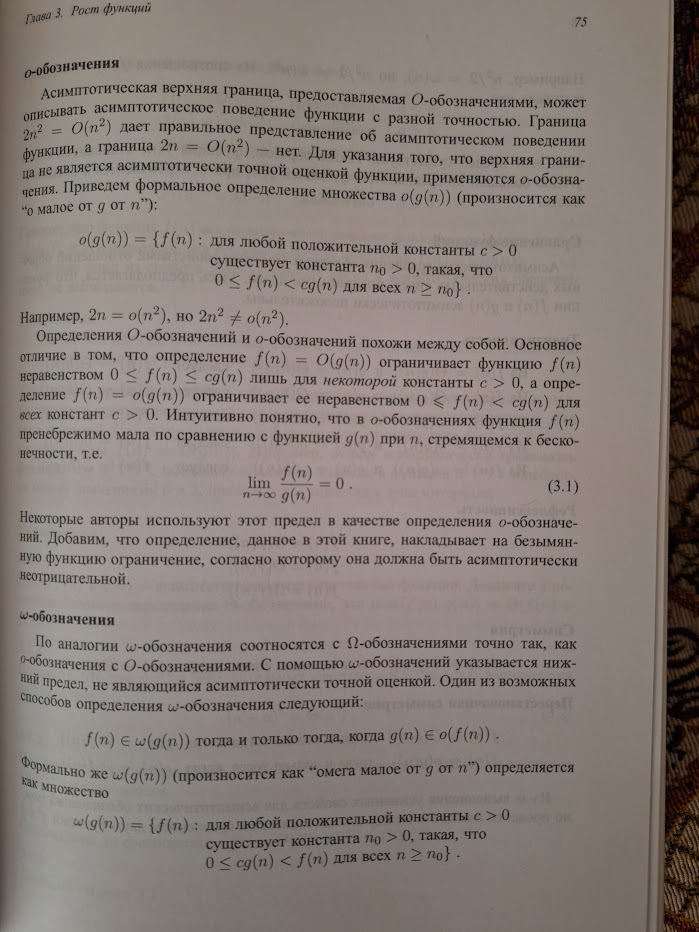
\includegraphics[scale=0.5]{img/perspective/wrong_input.jpg}
    \caption{Пример неправильно распознанного изображения: входное изображение}
    \label{perspective_wrong_input}
\end{figure}

\begin{figure}
    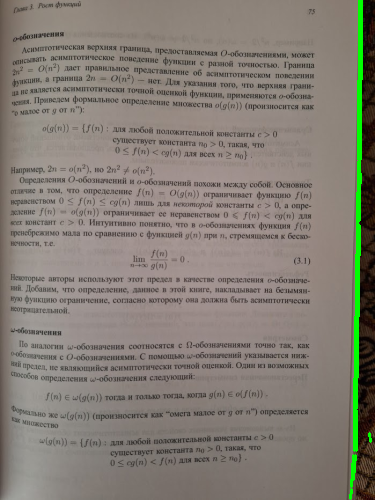
\includegraphics[scale=0.75]{img/perspective/wrong_output.png}
    \caption{Пример неправильно распознанного изображения: найденные контуры}
    \label{perspective_wrong_output}
\end{figure}